% Fig. M3 - Diagrama general del proceso de simulación
% Flowchart estándar (UML/ANSI): terminator, input/output (parallelogram),
% process (rectángulo), decision (diamond), predefined process (rectángulo
% con doble barra vertical). Paleta tomada de la referencia visual del usuario.
% Compile: pdflatex fig_m3_system_arch.tex
\documentclass[border=10pt]{standalone}
\usepackage[utf8]{inputenc}
\usepackage[T1]{fontenc}
\usepackage{amsmath}
\usepackage{xcolor}
\usepackage{tikz}
\usetikzlibrary{arrows.meta, positioning, calc, shapes.geometric}

% Paleta tomada de la imagen de referencia (cajas azul claro, borde azul medio)
\definecolor{boxfill}{RGB}{226, 237, 250}
\definecolor{boxborder}{RGB}{116, 156, 218}
\definecolor{arrowcol}{RGB}{70, 80, 90}

\begin{document}
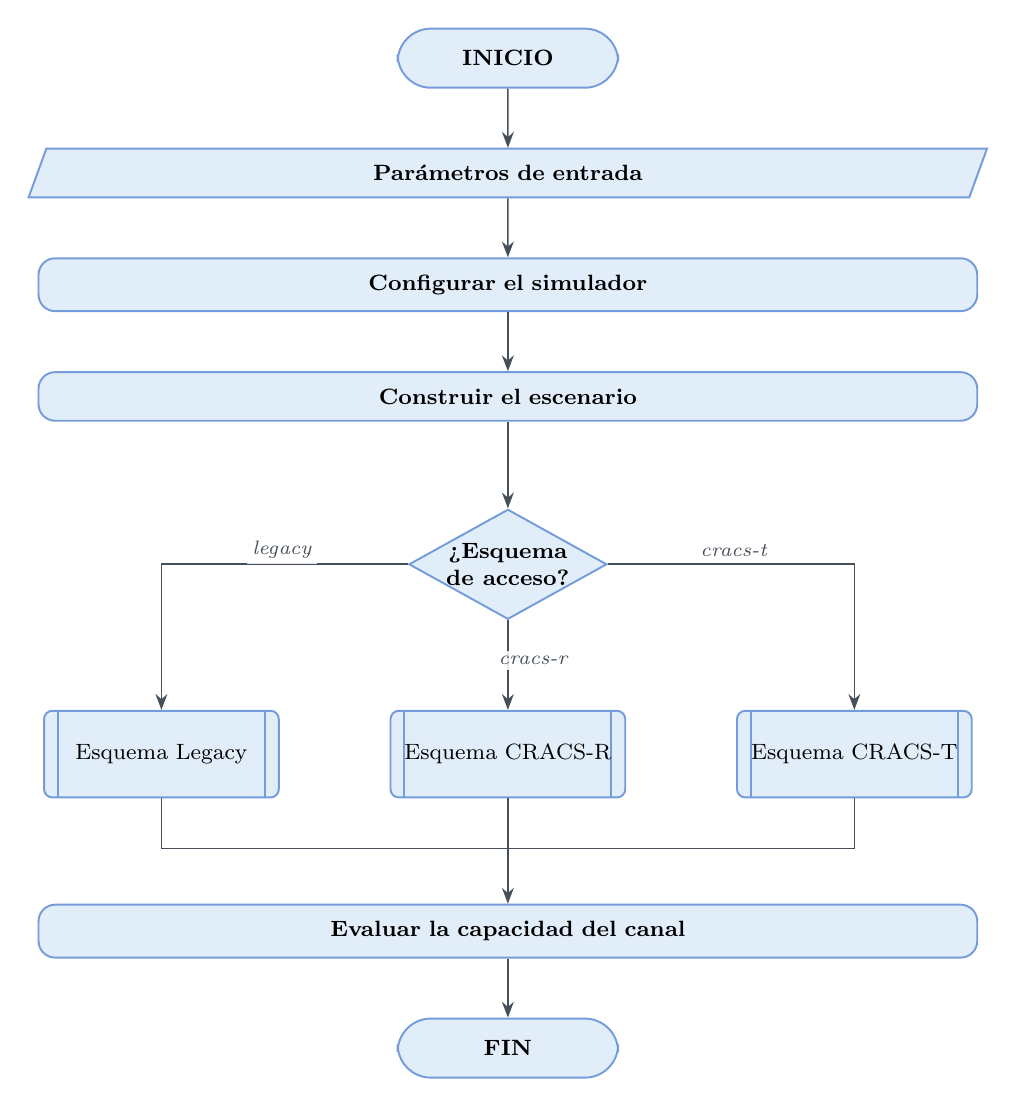
\begin{tikzpicture}[
    >=Stealth,
    font=\footnotesize,
    node distance=0.75cm,
    flowarrow/.style={->, semithick, draw=arrowcol},
    joinline/.style={-, semithick, draw=arrowcol},
    branchlabel/.style={font=\scriptsize\itshape, text=arrowcol, inner sep=2pt,
                        fill=white, fill opacity=0.85, text opacity=1},
    terminator/.style={rectangle, rounded corners=12pt,
                       draw=boxborder, fill=boxfill, line width=0.7pt,
                       minimum width=2.8cm, minimum height=0.75cm,
                       align=center, font=\footnotesize\bfseries},
    process/.style={rectangle, rounded corners=6pt,
                    draw=boxborder, fill=boxfill, line width=0.7pt,
                    text width=11.5cm, align=center,
                    font=\footnotesize, inner sep=6pt},
    decision/.style={diamond, draw=boxborder, fill=boxfill, line width=0.7pt,
                     aspect=1.8, minimum width=2.4cm, minimum height=1.1cm,
                     align=center, font=\footnotesize\bfseries, inner sep=0pt},
    iobox/.style={trapezium, trapezium left angle=70, trapezium right angle=110,
                  draw=boxborder, fill=boxfill, line width=0.7pt,
                  text width=11.3cm, align=center,
                  font=\footnotesize, inner sep=6pt},
    subroutine/.style={rectangle, rounded corners=3pt,
                       draw=boxborder, fill=boxfill, line width=0.7pt,
                       text width=2.7cm, minimum height=1.1cm,
                       align=center, font=\footnotesize, inner sep=4pt,
                       path picture={
                         \draw[boxborder, line width=0.7pt]
                           ([xshift=5pt]path picture bounding box.north west) --
                           ([xshift=5pt]path picture bounding box.south west);
                         \draw[boxborder, line width=0.7pt]
                           ([xshift=-5pt]path picture bounding box.north east) --
                           ([xshift=-5pt]path picture bounding box.south east);
                       }},
]

% ============================================================
% TITLE
% ============================================================

% ============================================================
% NODES (vertical flow)
% ============================================================
\node[terminator] (start) at (0, -0.3) {INICIO};

\node[iobox, below=of start] (input) {%
    \textbf{Parámetros de entrada}};

\node[process, below=of input] (config) {%
    \textbf{Configurar el simulador}};

\node[process, below=of config] (scenario) {%
    \textbf{Construir el escenario}};

\node[decision, below=1.1cm of scenario] (decision) {\textquestiondown Esquema\\de acceso?};

% Subroutines: spread horizontally below the decision
\node[subroutine] (legacy) at ($(decision.south) + (-4.4, -1.7)$)
    {Esquema Legacy};
\node[subroutine] (sara) at ($(decision.south) + (0, -1.7)$)
    {Esquema CRACS-R};
\node[subroutine] (new) at ($(decision.south) + (4.4, -1.7)$)
    {Esquema CRACS-T};

\node[process, below=3.6cm of decision] (evaluate) {%
    \textbf{Evaluar la capacidad del canal}};

\node[terminator, below=of evaluate] (end) {FIN};

% ============================================================
% MAIN VERTICAL FLOW
% ============================================================
\draw[flowarrow] (start) -- (input);
\draw[flowarrow] (input) -- (config);
\draw[flowarrow] (config) -- (scenario);
\draw[flowarrow] (scenario) -- (decision);

% ============================================================
% DECISION → 3 SUBROUTINES (clean L-shapes from west/south/east)
% ============================================================
\draw[flowarrow] (decision.west) -| (legacy.north);
\draw[flowarrow] (decision.south) -- (sara.north);
\draw[flowarrow] (decision.east) -| (new.north);

% Branch labels — placed on the horizontal segment / vertical segment
\node[branchlabel] at ($(decision.west) + (-1.6, 0.18)$) {legacy};
\node[branchlabel] at ($(decision.east) + (1.6, 0.18)$) {cracs-t};
\node[branchlabel] at ($(decision.south)!0.45!(sara.north) + (0.32, 0)$) {cracs-r};

% ============================================================
% 3 SUBROUTINES → EVALUATE  (T-junction merge, single arrowhead)
% ============================================================
\coordinate (mergeY) at ($(evaluate.north) + (0, 0.7)$);
\draw[joinline] (legacy.south) |- (mergeY);
\draw[joinline] (new.south)    |- (mergeY);
\draw[joinline] (sara.south)   -- (mergeY);
\draw[flowarrow] (mergeY) -- (evaluate.north);

% ============================================================
% TAIL
% ============================================================
\draw[flowarrow] (evaluate) -- (end);

\end{tikzpicture}
\end{document}
